\chapter{Alternative Design of Contact-free}

We analyzed the interaction mode on Apple Watch in last chaper, all the interaction method required two hands to be performed, except the voice interaction. Considering the actual scenario, if a user's hands are free to do anything, there is no abviouse reason to make things done on smart watches due to we have a powerful smart phone, moreover, to operate a phone acutally only needs one hand.
Therefore, this contact type of interaction on smart watch essentially isn't a stickiness interaction mode.
%上一章中我们分析了 Apple Watch 上的交互方式,
%除了语音交互外,这些方式都要求用户使用双手来完成整个交互。但实际场景中,如果用户双手空闲,
%则用户完全可以使用手机完成需要完成的事情,况且在屏幕适中的手机上完成交互也只需一直手。
%因此,这种交互模式从本质上就是一种不利于增加用户粘性的交互方式。
%考虑使用手表时的抬碗姿势,最自然的交互自然就是在抬碗时仅用一只手便能完成全部的交互行为。

\section{Interaction Pattern Design}

\subsection{Tap \& View Switch}

Tap and view switching oepration involving the following five operations: orinary tap, Force Touch tap, switch to left view, switch to right view, switch to previous view.
%点按与视图切换的操作一共涉及五个操作:普通点按、Force Touch 点按、切换到左视图、切换到右视图、切换到上一视图。

We design the alternative interaction of tap gesture to be two finger pinch, thumb pinch with the other four fingers can fully mapping all tap interaction, such as thumb with index finger can replace normal tap event, thumb with middle and ring finger can replace view switching, and thumb with little finger can replace back to previous view.
%单手手指的点击由两个两个手指的捏合操作来完成,拇指和其他四个手指的组合恰好能完成全部的点按交互,
%拇指和食指的点按来替代普通点击事件,拇指和中指、无名指的捏合实现视图的切换,拇指和小指的捏合则实现返回上级视图的功能。

Besides, pinch gesture with thumb and index finger can also simulize Force Touch, see more details in Section \ref{sub:force-touch-simu}.
%此外,拇指和食指的点按还能对 Force Touch 进行仿真,方法详见\ref{sub:force-touch-simu}一节。

\subsection{Swipe \& Continuous Adjustment}

% Slide is in fact two different scenarios and continuous expression is regulated by means of an interactive Digital Crown which,
% In general view slides able to view the contents of vertical adjustment, and when the interaction with the target selected for the slider (Slider Bar), whose value can be adjusted continuously.
%
Swipe and continue changes actrually belongs to Digital Crown interaction in different senarios. In General view down swipe senario, it can scroll view contents up and down; when the interactive object choose as slider bar, it also can adjust value continuesly.
%滑动与连续调节其实是由 Digital Crown 这一种交互手段在两种不同场景下表达,
%在一般视图下滑动时能够对视图内容进行纵向调节,而当交互目标选择为滑动器(Slider Bar)时,能够对其值进行连续调整。

% We can use two fingers of a single hand sliding to achieve this interaction. It refers to the slide of the thumb on the index finger,
% In the view by swiping up or down to achieve the selected interactive object, when closed over a slow slide to adjust the vertical display content,
% If the selected objects are interactive slider, then the slide is also possible to adjust the slider value.
%
We can implement this interaction by using two fingers pinch gesture on single hand, which means thumb slides on index finger, and if the interactive object is slide bar, then this kind of two fingers swipe can also regulate slide bar value.
%我们可以在单手上利用双指的相对滑动来实现这一交互。它是指由拇指在食指上的滑动,
%在视图内通过上下快速滑动来实现交互对象的选取,通过闭合时的的慢速滑动来调节纵向的内容展示,
%如果选取的交互对象是滑杆,那么这种滑动还能够调节滑动器的值。

\subsection{Force Touch Simulation}
\label{sub:force-touch-simu}

% An open source project Forcify \ cite {Huxpro: 2016ua} is a common framework for Web-side touch event,
% Any Web application in the Click event as a 3D Touch
% \ Footnote {Apple on the Force Touch technology on the iOS device to rename. }
% Processing, do not have the Force Touch enabled device using the method of touch event processing delay simulation.
% However, the delay time required for its handling events developers to customize, and the trigger Force Touch is a linear function of the intensity.
% To this end, we have to deal with this method is improved.
%
An open source project called Forcify\cite{Huxpro:2016ua} aims to develop an universe touch events handler framework, convert any Web App click events to 3D Touch Events\footnote{Apple rename Force Touch in iOS as 3D Touch.}. But the time handler need to customize by developer and the force touch simulator is a linear function. Therefore, this project needs to be improved.
%一项开源项目 Forcify \cite{Huxpro:2016ua} 是一个针对 Web 端触摸事件的通用框架,
%将任何 Web 应用里的点击事件作为 3D Touch
%\footnote{Apple 对 Force Touch 技术在 iOS 设备上重新命名。}
%进行处理,对不具备 Force Touch 功能设备采用触摸事件延时处理的方法进行模拟。
%然而,其处理事件的延时时间需要开发者自行定义,且触发 Force Touch 的力度是线性函数。
%为此,我们应对这个方法进行改进。

% First, touch events on the screen is divided into two stages, the first stage of a touch event treated as an ordinary touch touch events,
% Touch event for the second phase of the process Force Touch, and the use of trigger Force Touch DELAY time delay
% DURATION Force Touch represents the duration from minimum to maximum.
% The following study of these two constants are determined.
%
At first, we split touch events to two stage, the first stage is as normal touch events, the second stage is as Force Touch Events, and set contant DELAY to express the time delay of Force Touch, and DURATION to express the time duration of Force Touch from minimum to maximum.
Now we focus on this two constants value.
%首先,对屏幕上的触摸事件划分为两个阶段,第一个阶段的触摸事件处理为普通触摸的触摸事件,
%第二个阶段的触摸事件处理为 Force Touch,并使用 DELAY 表示触发 Force Touch 的时间延时,
%DURATION 表示 Force Touch 从最小值到最大值的持续时间。
%下面考察这两个常量的取值。

% In AugmentedTouch \ cite {Changkun: 2016} project, we carried out a user survey and released containing 16 users,
% 4 different hand position, implemented a total of 61440 times the screen click on the data set.
% In this data set, click on the screen each time the user's finger is recorded on the screen of the residence time, Figure \ ref {fig: result} shows the distribution of this 61440 views residence time.
%
In AugmentedTouch Project\cite{Changkun:2016}, we applied a user study and published a dataset contains 16 users of 4 different posture, altogether contains 61440 times tap data. In this dataset, we record the time of user's finger stay on screen and Figure \ref{fig:result} shows its distribution.
%在 AugmentedTouch \cite{Changkun:2016} 项目中,我们实施了一个用户调研并发布了一个包含 16 名用户、
%使用 4 种不同的手姿、共实施 61440 次屏幕点击的数据集。
%在这个数据集中,每次的屏幕点击均记录了用户的手指在屏幕上的停留时间,图\ref{fig:result}展示了这 61440 次点击的停留时间的分布。

\begin{figure}[H]
    \kaishu
    \centering
    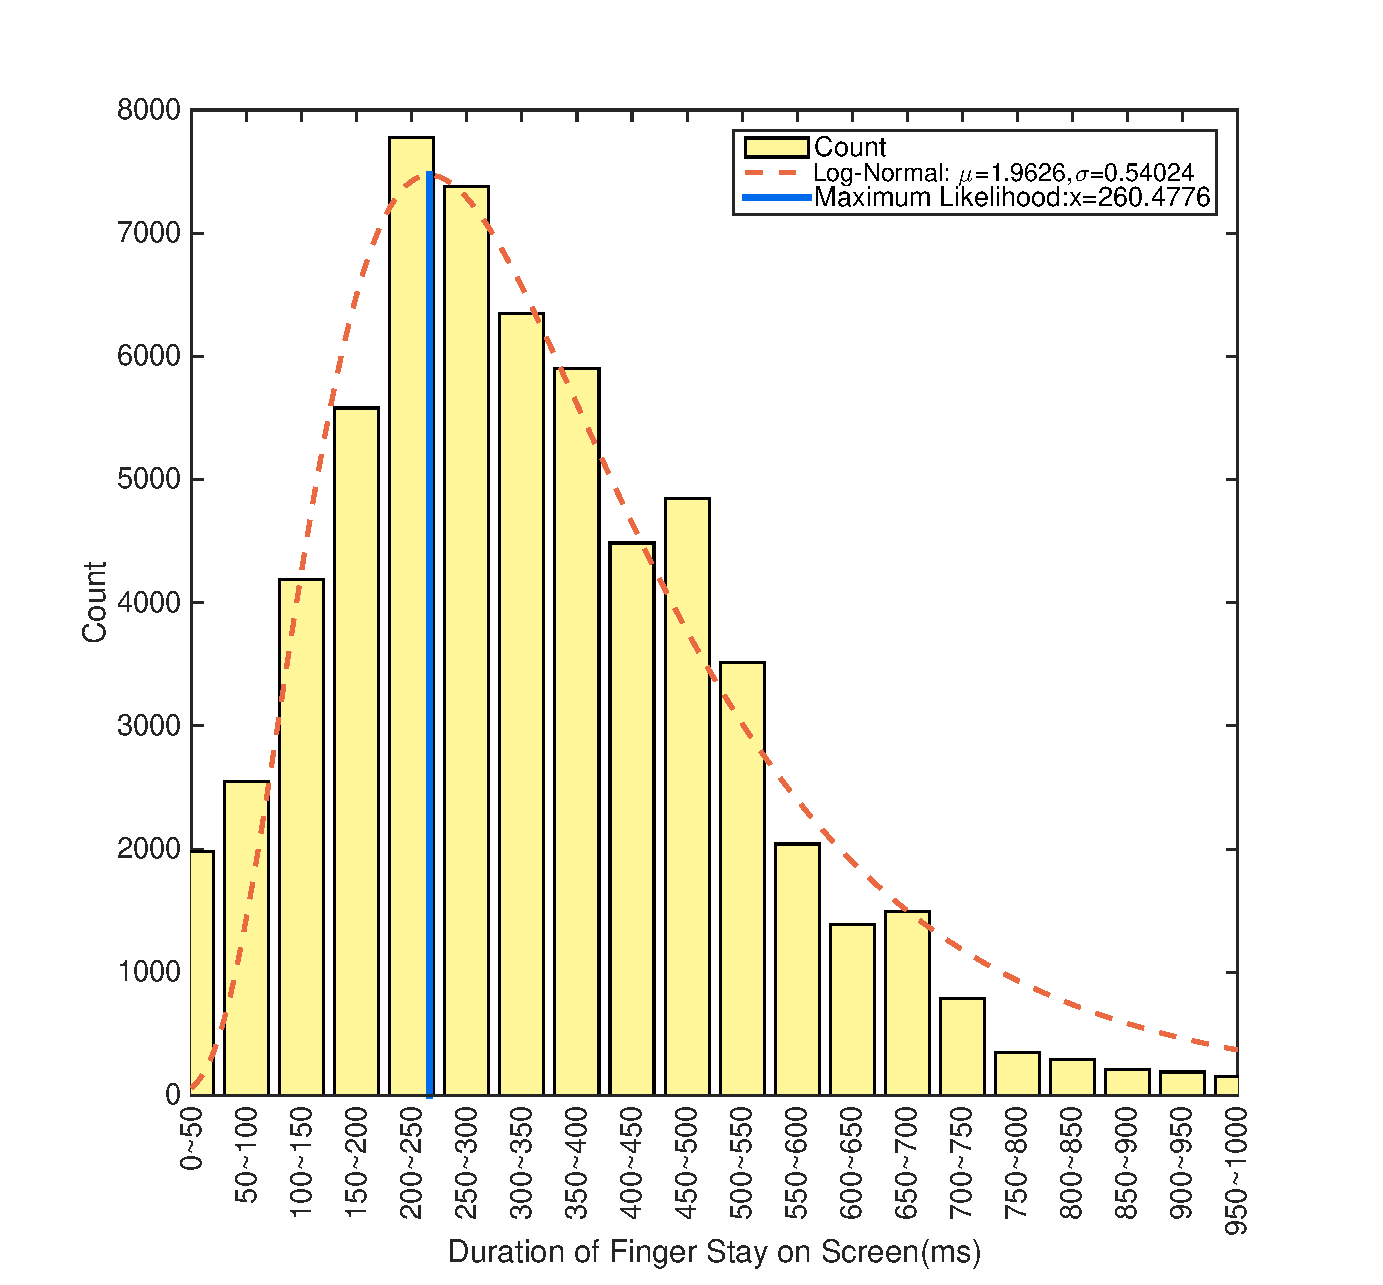
\includegraphics[width=0.5\textwidth]{figures/count-result}
    \caption{\kaishu Statistics of finger stay on screen}
    \label{fig:result}
\end{figure}

As it shows the discribution on Figure \ref{fig:result} we can get the time of a finger stay on a screen mainly focus on 260ms, obey to log-normal distribution.
In this regard, we could assume the average time of finger stay on touch screen is 250 ms, so DELAY equals 250 ms;
In addition, we set the total duration is five times of the ordinary touch events time, so DURATION equals 1000 ms;
Then to trigger the Force Touch user need stay finger on touch screen longer than 1.25 seconds.
Considering human's finger presure of touch, we also assume the intensity of the rate of force value is linear, then we can ensure the entire curve is a smooth curve.

%从图\ref{fig:result} 的分布上我们可以看出,手指在屏幕上的停留时间主要集中在 260 ms 前后,呈对数正态分布。
%对此,我们不妨将手指在屏幕上的平均停留时间设为 250 ms,故 DELAY 的值为 250ms;
%另外,设 Force Touch 总持续时间为普通触摸事件的五倍,故 DURATION 的值为 1000ms;
%这时触发 Force Touch 操作所需要的总时间为 1.25 秒。
%对 Force Touch 而言,考虑人类手指的按压力度变化,我们设其力度的变化率线性变化,
%这时能保证整条力度变化曲线为光滑曲线。

In conclution, let the time of pressing to be $t_{\text{press}}$, and Force Touch can be simulate by a formula \ref{formal:delay}.
%综上所述,记在一次按压中的按压时间为 $t_{\text{press}}$,
%则 Force Touch 可以使用公式\ref{formal:delay}进行模拟:
\begin{equation}
v_{F} =
    \begin{cases}
        0    & \mbox{if $t_{\text{press}} < \text{DELAY}$} \\
        \left(\frac{t_{\text{press}}-\text{DELAY}}{\text{DURATION}}\right)^{2}
             & \mbox{if 0 < $t_{\text{press}}-\text{DELAY} < \text{DURATION}$} \\
        1    & \mbox{Otherwise}
    \end{cases}
\label{formal:delay}
\end{equation}

Among the formula, $v_{F}$ represents the presure value, DELAY = 250, DURATION = 1000, both in milliseconds(ms), as shown in Figure \ref{fig:ft-fig}.
%其中,$v_{F}$表示模拟的压力值,DELAY = 250,DURATION = 1000,两者单位为毫秒(ms),图像如图\ref{fig:ft-fig}所示。

\begin{figure}[htbp]
\centering
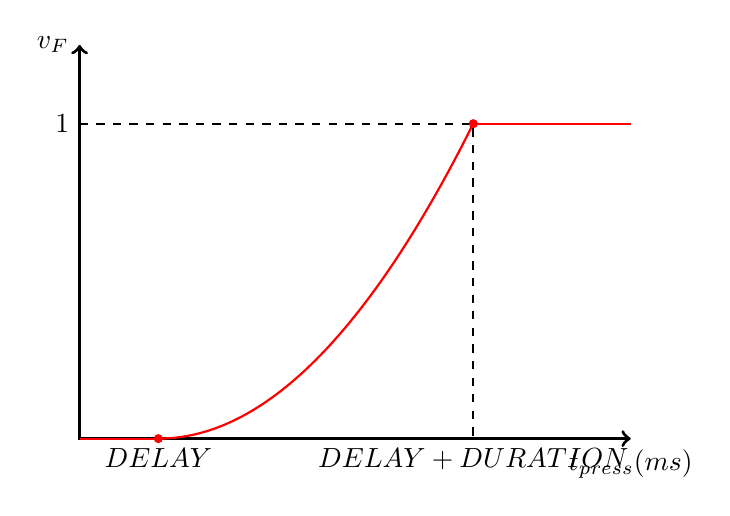
\begin{tikzpicture}[domain = 0:5, xscale = 1, yscale = 1]
    \draw [very thick, <->] (0, 5) node [left] {$v_{F}$}
             -- (0, 0) -- (7.0, 0) node [below] {$t_{\text{press}}\text{(ms)}$};

    \draw[domain=0:1, thick, smooth, color=red] plot(\x, 0);
    \draw[domain=1:5, thick, smooth, color=red] plot(\x, {0.25*(\x-1)^2});
    \draw[domain=5:7, thick, smooth, color=red] plot(\x, 4);

    \node[below] at (1.0, 0.0) {$\text{\tiny DELAY}$};

    \draw[thick, dashed] (0, 4) node [left] {1}
           -- (5,4) -- (5,0) node [below] {$\text{\tiny DELAY+DURATION}$};

    \draw[fill,color=red] (1,0) circle [radius=0.05];
    \draw[fill,color=red] (5,4) circle [radius=0.05];
\end{tikzpicture}
\caption{Force Touch functional image}
\label{fig:ft-fig}

\end{figure}

\subsection{Haptic Feedback Design}

According to the developer documentation of watchOS\footnote{watchOS version stay on 2.2 when this thesis finished.}, Haptic Engine can express several types, as its illustrate on Code \ref{lst:haptic-define}.
%在 watchOS 中\footnote{本文写成时的 watchOS 版本为 2.2。},
%根据开发文档\cite{WatchGuide:2016}显示Haptic Engine 一共能表达代码\ref{lst:haptic-define}所示的几种类型。

\begin{lstlisting}[
    language={Swift},
    caption={\kaishu Types of Haptic feedback},
    label={lst:haptic-define}
]
public enum WKHapticType : Int {
    case Notification
    case DirectionUp
    case DirectionDown
    case Success
    case Failure
    case Retry
    case Start
    case Stop
    case Click
}
\end{lstlisting}

% Success, Failure, Retry Haptic three types are native to the operating results of the implementation of interactive feedback,
% So we will set to Success alternative interaction and feedback successfully completed operations after the implementation, Failure corresponds to fail.
% When the original interactive born, Retry only after the failure to enter the password when special circumstances,
% Feedback may wish to use this case still represented Failure, first to keep this type of feedback to be used for other interactions.
Success, Failure, Retry type of Haptic feedback are native results in watch operation.
Then we set Success, Failure as same as its original function, but the context of Retry is basiclly as same as Failure, so we keep this feedback for the future.
%Success、Failure、Retry 三个 Haptic 类型均为对原生交互的操作执行结果的反馈,
%于是我们将 Success 设置为备择交互中执行完操作且成功后的反馈,Failure 则对应为失败。
%在原生交互时,Retry 只用于在输入密码时失败后的特殊情况,
%不妨将此种情况的反馈依然用 Failure 表示,先保留此反馈类型,以便用于其他交互。

% Notification Notification for reminder in the sleep state, not be modified;
% DirectionUp and DirectionDown native interaction Digital Crown feedback reminder to rotate when the top and bottom,
% In this regard we also inherit this feedback design, and extended to the spin, when adjusted to the maximum value, execution DirectionUp feedback,
% Conversely execution DirectionDown feedback.
Notification feedback still needs to present notification feedback, so we don't change its design; DirectionUp and DirectionDown only happens on Digital Crown scroll up and down in the end, so we follow this function to two fingers swipe, when value comes to the maximum value, use DirectionUp feedbacl and  vice versa.
%Notification 用于在休眠状态下的通知提醒,不对其进行修改;
%DirectionUp 和 DirectionDown 是原生交互中 Digital Crown 旋转到顶端和底端时的反馈提醒,
%对此我们同样继承此反馈设计,并扩展到数值调节中,当调整到数值最大值时,执行 DirectionUp 反馈,
%反之执行 DirectionDown 反馈。

Start, Stop, Click and Retry this four type of feedback can suiteablely for thumb with index, middle, ring finger pinch (three) and Force Touch operate, which means feedback of Click is for normal tap, feedback of Stop is for Force Touch, feedback of Start is for view switching to next, and feedback of Retry just right for view switching to previous.
%Start、Stop、Click 和 Retry 四个反馈类型恰好可以对拇指与食指、中指、
%无名指捏合点击与 Force Touch 的四个个不同操作进行对应,
%即 Click 表示普通点击事件,Stop 表示 ForceTouch 操作,
%Start表示切换到下一视图,Retry 恰好用于切换到上一视图的提示反馈。

\section{Completeness of Alternative Design}
\label{sec:completeless}

\begin{figure}[H]
    \kaishu
    \centering
    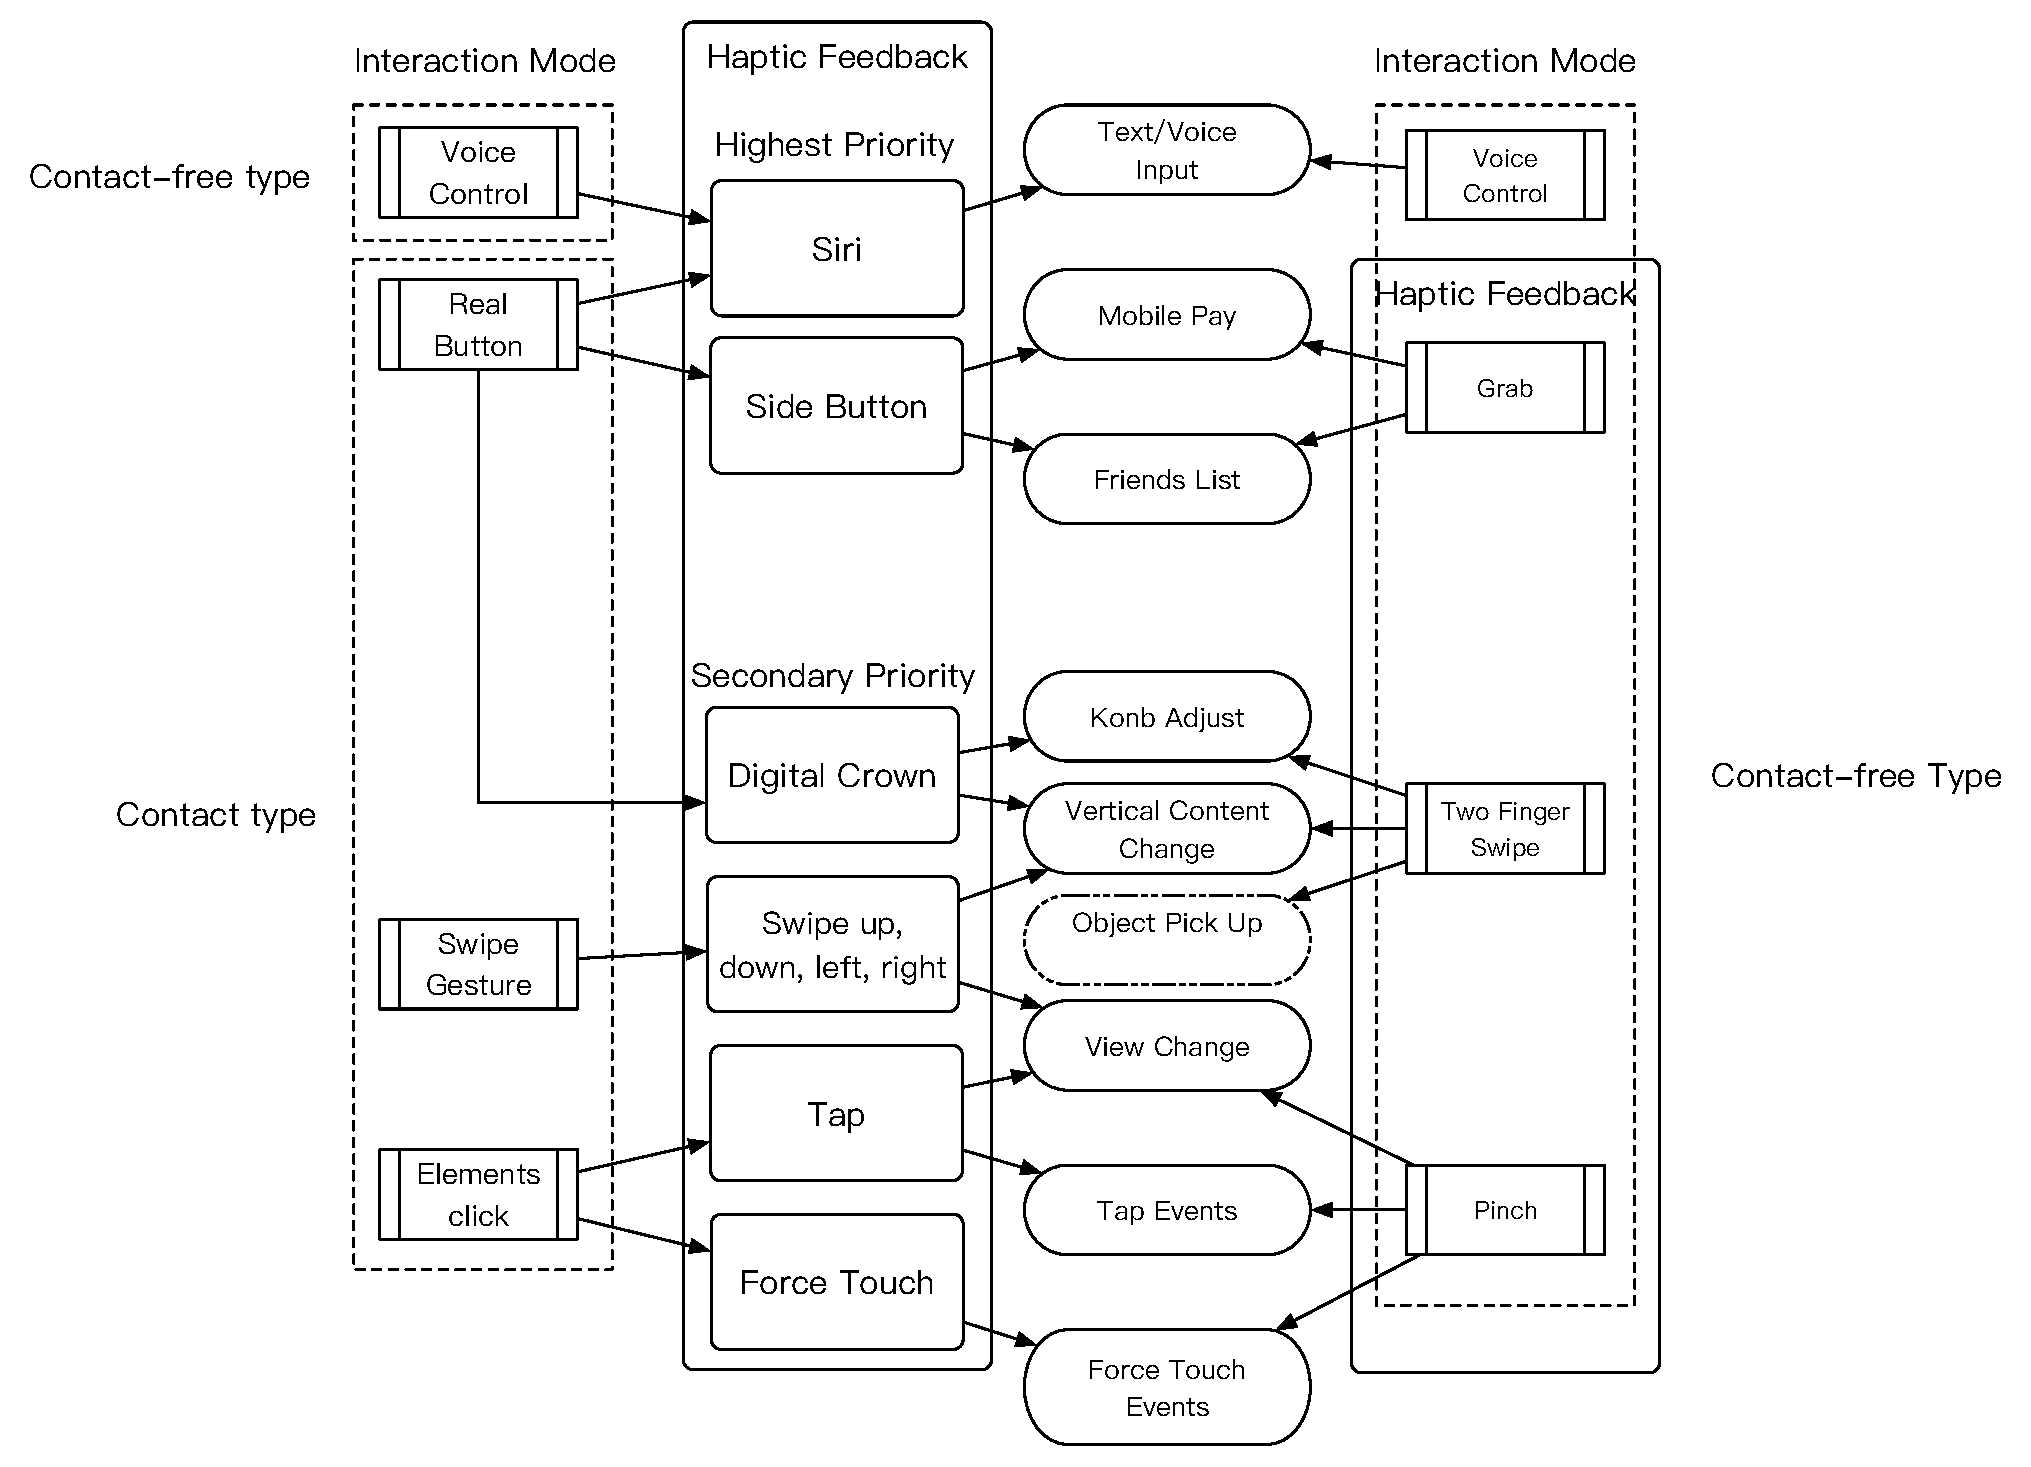
\includegraphics[width=0.6\textwidth]{figures/interaction-en}
    \caption{\kaishu Summary of Contact-free Interaction}
    \label{fig:interaction}
\end{figure}

In this chapter, we fully redesigned the interaction mode on Apple Watch, it simplifies the interaction logic between elements, as a summary we list the design logic in Figure \ref{fig:interaction}.
This design, combine with the Haptic feedback, convert the basic tap, swipe, Digital Crown, Force Touch and etc. native watch interaction to a contact-free gesture interaction. It simplefied ten native interaction with two-step logic to only eight alternative interaction with sigle-step logic, eliminated contact-required interaction.
%本章中我们全面地对 Apple Watch 上的交互进行了重新设计,
%简化了元素与元素之间的交互逻辑,作为小结,如图\ref{fig:interaction}。
%在此套备择设计中,我们将原有的两层交互逻辑中十种不同交互逻辑通过简化为单层交互逻辑的八种,
%并且消除了接触式交互这一限制。

As illustrate in Figure \ref{fig:interaction}, this interaction scheme is completeless, which means we archived all the funtion without original interaction method.
%从图\ref{fig:interaction}中我们容易看出,备择设计在交互上是完备的,即从另一个角度实现了原交互的全部功能。

\cleardoublepage
